% -*- coding: UTF-8 -*-
% vim: autoindent expandtab tabstop=4 sw=4 sts=4 filetype=tex
% vim: spelllang=de spell
% chktex-file 27 - disable warning about missing include files

\section{Komponenten}
\label{sec:main-components}

Ausgehend von den Anforderungen (siehe~\autoref{sec:requirements}) können einzelne
Komponenten der Applikation abgeleitet werden. Einzelne Teile davon wurden
schon durch die Vision (siehe~\autoref{subsec:requirements:vision}) definiert
beziehungsweise aus dieser gewonnen.

Dieser Prozess entspricht nicht direkt dem Vorgehen
gemäss~\cite{larman_applying_2004} beziehungsweise dem UP, der Autor dieser
Projektarbeit ist jedoch der Ansicht, dass dieser Abschnitt eine Brücke
zwischen Anforderungen und der (Software-) Modellierung bildet. Zudem bietet
dieser Abschnitt eine relativ bildliche Beschreibung, was dem Verständnis des
Gesamtkonzeptes sicher zuträglich ist. Am ehesten entspricht dieser Abschnitt
den Komponenten-Diagrammen in~\cite[S. 653 bis 654]{larman_applying_2004}.

Die Applikation besteht aus zwei Applikationen: Einem \textit{Player},
welcher dem Abspielen von Echtzeit-Animationen dient, sowie einem \textit{Editor},
welcher der Erstellung und Verwaltung von Echtzeit-Animationen dient.

\subsection{Player}
\label{subsec:main-components:player}

Der \textit{Player} liest die vom \textit{Editor} exportierten
Echtzeit-Animationen. Er bietet vor dem Abspielen die Auswahl der Auflösung,
des Seitenverhältnisses, Antialiasing und ob die Animation im Vollbild-Modus
abgespielt werden soll.

\subsection{Editor}
\label{subsec:main-components:editor}

Der \textit{Editor} erlaubt das Erstellen und Bearbeiten von
Echtzeit-Animationen. Diese können schliesslich inklusive den
dazugehörigen Dateien, wie zum Beispiel Bitmaps oder Modellen, exportiert
werden.

\begin{figure}[H]
    \centering
    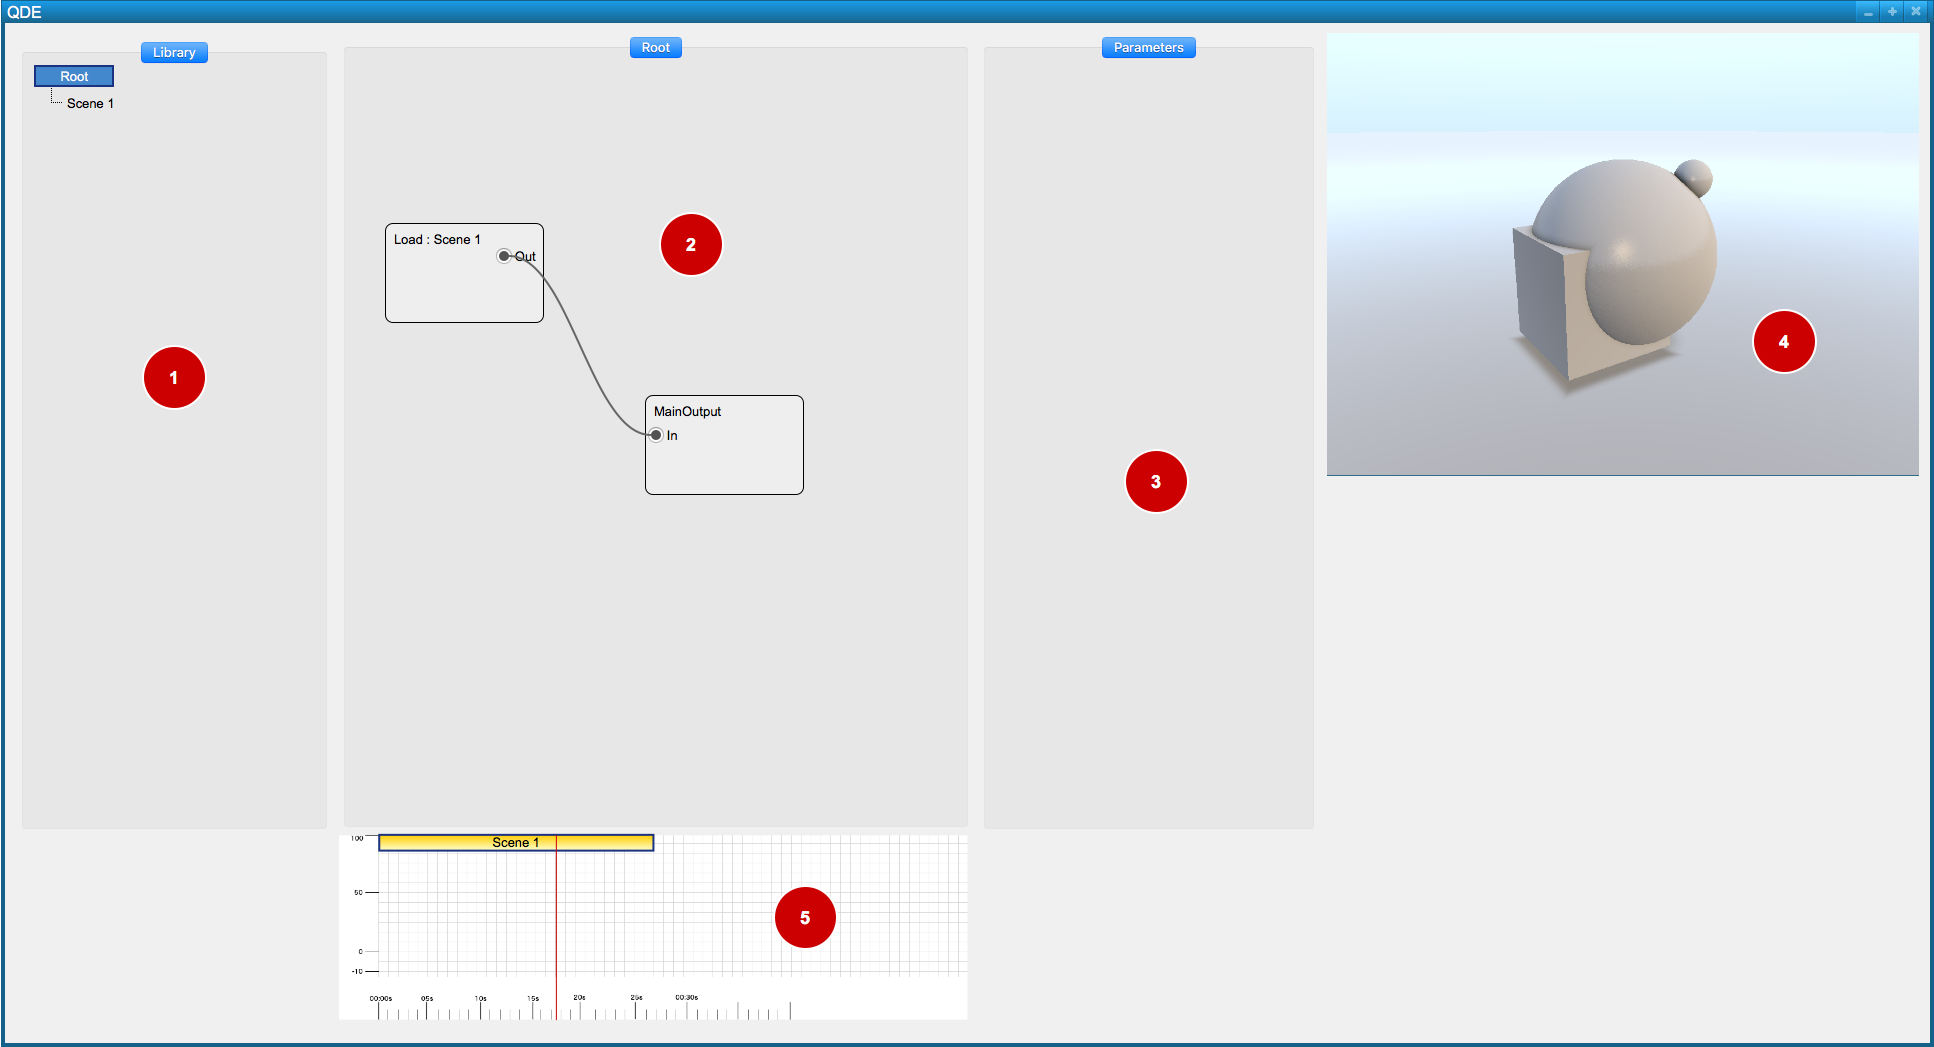
\includegraphics[width=0.9\textwidth]{img/editor_components.png}
    \caption{Einzelne Komponenten des
        Editors}\label{fig:main-components:editor:editor-components}
\end{figure}

Abbildung~\ref{fig:main-components:editor:editor-components} zeigt die
einzelnen Komponenten des Editors. Nachfolgend findet sich eine Beschreibung
dieser.

\subsubsection{Bibliothek}
\label{ssubsec:main-components:editor:library}

Das Element~\img[20pt]{img/editor_component_1.png} in
Abbildung~\ref{fig:main-components:editor:editor-components} zeigt die
(Szenen-) Bibliothek. Diese beinhaltet alle Szenen einer Echtzeit-Animation.
Eine Szene ist dabei eine Menge von Knoten und Kanten. Es können neue Szenen
angelegt und auch bestehende Szenen gelöscht werden. Wird ein neues Projekt
erstellt, so verfügt dieses immer über die ``Root''-Szene. Diese beinhaltet den
Haupt-Ausgabeknoten des Graphen, welcher schliesslich zum Abspielen evaluiert
wird, und kann nicht gelöscht werden. Wird eine Szene mit der Maus angewählt,
so wird deren Inhalt im Graphen dargestellt.

\subsubsection{Graph}
\label{ssubsec:main-components:editor:graph}

Das Element~\img[20pt]{img/editor_component_2.png} in
Abbildung~\ref{fig:main-components:editor:editor-components} zeigt den Graphen
einer Szene. Dieser beinhaltet sämtliche Knoten einer Szene. Mittels
Kontextmenü können neue Knoten eingefügt und bestehende Knoten gelöscht werden.
Wird ein Knoten angewählt, so wird dieser einerseits im
Rendering-Ansichtsfenster dargestellt, andererseits werden dessen Eigenschaften
im Parameter-Fenster angezeigt.

Folgende Typen von Knoten sind geplant:
\begin{itemize}
    \item \textbf{Scene}\\
        Eine Menge von Knoten und Kanten.

    \item \textbf{TimelineClip}\\
        Eine Szene, welche in der Zeitachse platziert werden kann.

    \item \textbf{Model}\\
        Ein Objekt, wie zum Beispiel ein Würfel oder eine Kugel.

    \item \textbf{Camera}\\
        Eine Kamera, welche die Sicht auf eine Szene erlaubt.

    \item \textbf{Light}\\
        Ein Licht, welches in einer Szene platziert wird und welches für
        Beleuchtung dieser sorgt.

    \item \textbf{Material}\\
        Definiert Material-Eigenschaften eines Objektes, zum Beispiel ob dessen
        Oberfläche matt oder reflektierend ist.

    \item \textbf{Operator}\\
        Bietet eine Operation wie zum Beispiel die Gruppierung von zwei
        Modellen oder die Verdrehung eines Modelles.

    \item \textbf{Effect}\\
        Ein Nachbearbeitungs-Effekt (postprocessing-effect) wie zum Beispiel
        Bewegungsunschärfe oder Bloom.
\end{itemize}

\subsubsection{Parameter}
\label{ssubsec:main-components:editor:parameters}

Das Element~\img[20pt]{img/editor_component_3.png} in
Abbildung~\ref{fig:main-components:editor:editor-components} zeigt die
Parameter des aktuell gewählten Knoten im Graphen. Neben jedem Parameter
befindet sich eine Schaltfläche zum Setzen von Schlüsselbildern (Keyframes) in
der Zeitachse (Timeline). Wird die Schaltfläche betätigt, so wird bei dem
aktuell ausgewählten Zeitpunkt der Zeitachse ein Schlüsselbild gesetzt.

\subsubsection{Rendering}
\label{ssubsec:main-components:editor:rendering}

Das Element~\img[20pt]{img/editor_component_4.png} in
Abbildung~\ref{fig:main-components:editor:editor-components} zeigt das
Rendering-Ansichtsfenster. Dieses stellt den Inhalt des aktuell gewählten
Knotens dar. Die Art des Knotens ist dabei nicht beschränkt, es kann dies eine
Szene, aber zum Beispiel auch ein einzelnes Modell sein. Es wird immer der
gesamte vorhergehende (Teil-) Baum des Knotens evaluiert.

\subsubsection{Zeitachse}
\label{ssubsec:main-components:editor:timeline}

Die Zeitachse wird mit~\img[20pt]{img/editor_component_5.png} in
Abbildung~\ref{fig:main-components:editor:editor-scene1} dargestellt.  Sie
bildet das zeitliche Geschehen einer Echtzeit-Animation ab. Alle Knoten vom Typ
Timeline-Clip werden am oberen Rand des Fensters in deren zeitlicher
Reihenfolge abgebildet. Wird im Graph ein Knoten mit animierten Parametern
angewählt, so sind diese ersichtlich. Vertikal wird der Wertebereich,
horizontal die Zeitachse in Sekunden dargestellt. Ein vertikal verlaufender,
roter Marker zeigt die aktuelle zeitliche Position der Echtzeit-Animation an.

Abbildung~\ref{fig:main-components:editor:editor-scene1} zeigt ein Beispiel,
wie eine typische Szene mit animierten Parametern aussehen könnte. Der
Übersicht halber werden nur der Graph, die Parameter sowie die Zeitachse
dargestellt.

\begin{figure}[H]
    \centering
    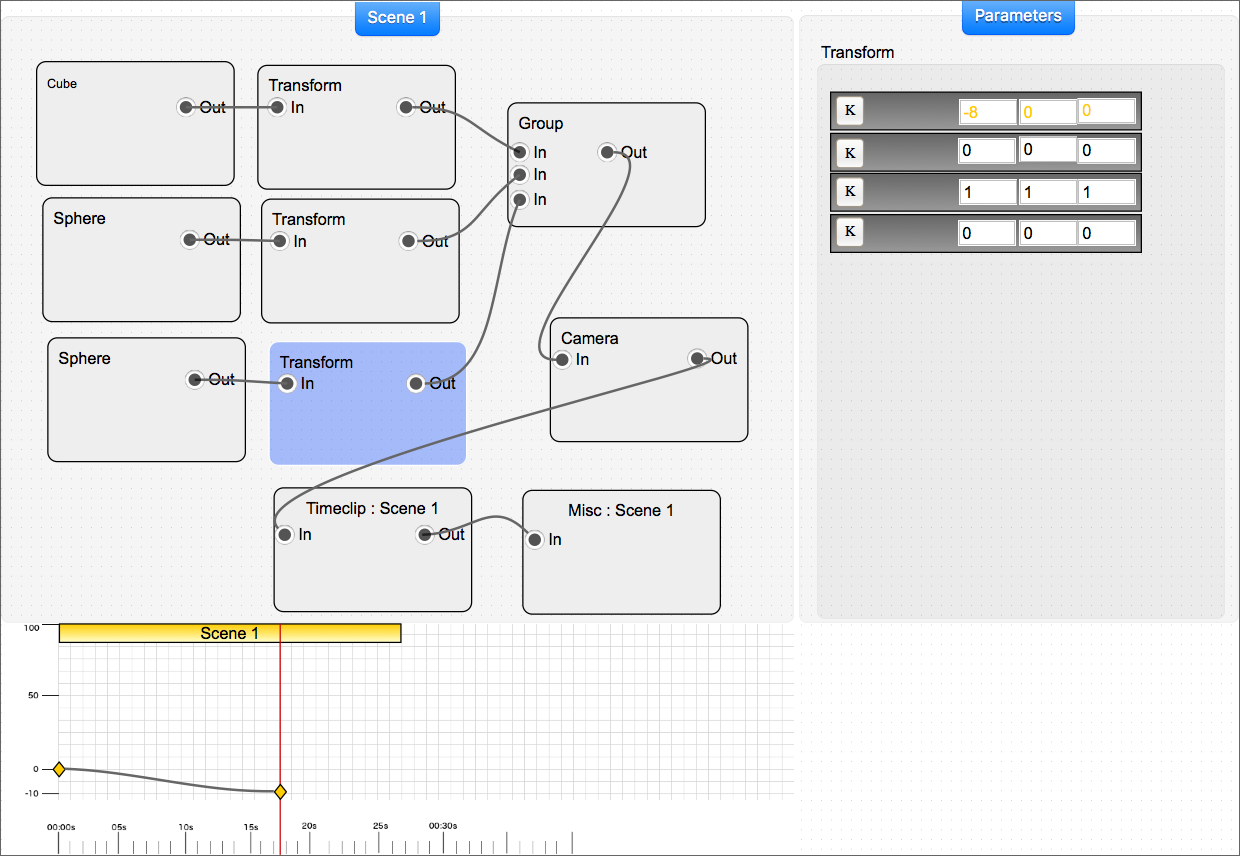
\includegraphics[width=0.9\textwidth]{img/editor_scene1_details.png}
    \caption{Graph, Parameter und Zeitachse einer Beispiel-Szene innerhalb des
        Editors.}\label{fig:main-components:editor:editor-scene1}
\end{figure}
